\chapter{Magneto-static magnetic scalar potential}

\section{Kinematics}
We consider a magneto-elastic solid body $\mathcal{B}_0$ in a three-dimensional Euclidean space that is initially in stress-free configuration, not subjected to any mechanical or magnetic field loads. On application of a magnetic load defined by a magnetic field $\mathbb{H}$ and an associated magnetic induction $\mathbb{B}$ and magnetization vector $\mathbb{M}$, in the absence of any mechanical load, the body will undergo some deformation due to this magnetic load. This phenomenon is referred to as \textit{magnetostriction}. Let the resulting deformed configuration from the magnetostriction be denoted as $\mathcal{B}_t$. This configuration will depend on the choice of the initial magnetic field $\mathbb{H}$. \par 
Let any point in the reference configuration $\mathcal{B}_0$ be identified by the position vector $\mathbf{X}$ and it's position in the deformed configuration $\mathcal{B}_t$ be given as $\mathbf{x} = \bm{\varphi} (\mathbf{X})$. The field $\bm{\varphi}$ is a one-to-one mapping describing the deformation of the body. The associated deformation gradient $\mathbf{F}$ relative to $\mathcal{B}_0$ is defined as $\mathbf{F} := \nabla_0 \bm{\varphi}$ and it's determinant is $J = \text{det}\mathbf{F} > 0$ (non-negative to avoid material self-penetration). The gradient w.r.t. the reference configuration $\mathcal{B}_0$ is denoted as $\nabla_0$ and the gradient w.r.t. the deformed configuration $\mathcal{B}_t$ be denoted as $\nabla$. The magnetic vector fields in the deformed configuration are denoted as $\mathbbm{b}, \mathbbm{h}$ and $\mathbbm{m}$.\par 

\begin{figure}[h]
\centering 
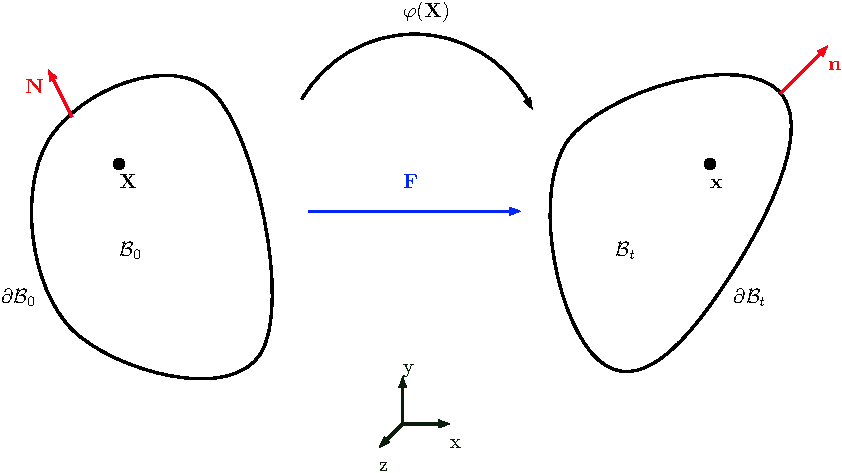
\includegraphics[width=0.65\textwidth]{kinematics_potato.pdf}
\caption{Kinematics}
\label{fig:1.1}
\end{figure} 

\section{Balance equations}
\subsection{Magnetic balance laws}
In the absence of any deformation ($\mathbf{F} = \mathbf{I}$), the magnetic quantities $\mathbbm{b}, \mathbbm{h}, \mathbbm{m}$ are related by the standard formula
\begin{equation}
\mathbbm{b} = \mu_0 (\mathbbm{h} + \mathbbm{m}),
\label{eq:1.1}
\end{equation}
where $\mu_0 = 4\pi \times 10^{-7} \text{Hm}^{-1}$ is the magnetic permeability in vacuum. \par 
For the case of time-independent problems and in the absence of external currents, from the Ampere's law we have \cite{KANKANALA} 
\begin{equation}
\text{curl} (\mathbbm{h}) = \nabla \times (\mathbbm{h}) = \mathbf{0}.
\label{eq:1.2}
\end{equation}
For the case of magneto-statics (absence of time varying electromagnetic fields), from the assumption of the absence of magnetic monopoles we have \cite{KANKANALA}\begin{equation}
\text{div}(\mathbbm{b}) = \nabla \cdot \mathbbm{b} = 0.
\label{eq:1.3}
\end{equation}
Both the Equations \eqref{eq:1.2} and \eqref{eq:1.3} are the specializations of Maxwell's equations. Equation \eqref{eq:1.1} defines the third vector field when one field is used as an independent variable and the other field is provided by an appropriate constitutive law. 

\subsection{Mechanical balance laws}
The balance law for mass conservation is given as 
\begin{equation}
\frac{d\rho}{dt} + \nabla \cdot [\rho \mathbf{\dot{x}}] = 0,
\end{equation}
where $\rho$ is the mass density in $\mathcal{B}_t$. \par 
From the balance law for linear momentum assuming that the inertial effects are negligible, we have the equilibrium equation 
\begin{equation}
\text{div} \bm{\sigma} + \bm{b}_t = \mathbf{0} \ \ \text{in} \ \mathcal{B}_t,
\end{equation}
where $\bm{\sigma}$ is the Cauchy stress tensor and $\bm{b}_t$ is the body load per unit current volume. The balance of angular momentum leads to the requirement that $\bm{\sigma}$ is symmetric. 

\section{Boundary conditions}
In order to formulate a boundary-value problem we need constitutive laws in which $\bm{\sigma}$ and $\mathbbm{b}$ are given in terms of the variables $\mathbf{F}$ and $\mathbbm{h}$. Additionally, appropriate boundary conditions must be satisfied by the fields $\mathbbm{b}, \bm{\sigma}$ and $\bm{\varphi}$. At a bounding surface of the material body in the deformed configuration, the vector fields $\mathbbm{b}$ and $\mathbbm{h}$ satisfy the standard jump conditions
\begin{equation}
\mathbf{n} \cdot \llbracket \mathbbm{b} \rrbracket = 0, \ \ \mathbf{n} \times \llbracket \mathbbm{h} \rrbracket = \mathbf{0} \ \ \text{on} \ \partial\mathcal{B}_t,
\label{eq:1.4}
\end{equation}
where the square brackets indicate a jump across the surface and $\mathbf{n}$ is the outward pointing unit normal vector to the surface in the deformed configuration $\mathcal{B}_t$. These boundary conditions enforce that the tangential component of the magnetic field, as well as the normal component of the magnetic induction, remain continuous on the boundary \cite{pelteret2016}.

\section{Magnetic scalar potential (MSP) formulation}
The magnetic field quantities ($\mathbbm{b}, \mathbbm{h}, \mathbbm{m}$) are all discontinuous over boundaries and material interfaces: $b_{1t} \neq b_{2t}, h_{1n} \neq h_{2n}$ when $\mu_1 \neq \mu_2$ (where $t$ and $n$ denote the tangential and normal components, respectively). These discontinuities are difficult to model using the finite element method simulations. Thus, a fictitious quantity such as the magnetic scalar potential $\phi$ is used in solving the magneto-elastic problems using FEM. The magnetic scalar potential formulations can be used only in the case where there are no free currents in the domain. We define a scalar potential related to the curl-free magnetic field by \cite{pelteret2016}
\begin{equation}
\mathbbm{h} := -\nabla \phi \ \ \text{in} \ \mathcal{B}_t. 
\label{eq:1.5}
\end{equation}
The continuity condition associated with $\phi$ is 
\begin{equation}
\llbracket \phi \rrbracket = 0 \ \ \text{on} \ \partial\mathcal{B}_t.
\end{equation}
The magnetic induction vector $\mathbbm{b}$ is modelled in terms of magnetic field $\mathbbm{h}$, taking $\mathbbm{h}$ as the independent field
\begin{equation}
\mathbbm{b} = \mathbbm{b}(\mathbbm{h}).
\end{equation}
We consider the magnetization ($\mathbbm{m}$) and the magnetic field $(\mathbbm{h})$ are aligned. For a material with relative permeability $\mu_r$ we have
\begin{equation}
\mathbbm{h} + \mathbbm{m} = \mathbbm{h} + (\mu_r - 1)\mathbbm{h} = \mu_r \mathbbm{h}.
\end{equation}
The relation for the magnetic induction in terms of the magnetic field using the above relation is
\begin{equation}
\mathbbm{b} = \mu_0 \mu_r \mathbbm{h}.
\label{eq:1.7}
\end{equation}

\section{Variational formulation}
In this section, we will derive the axisymmetric weak form of the magnetic balance law:
\begin{equation}
 \text{div}\mathbbm{b} = 0,
 \end{equation} 
with the body symmetric about the Y-axis in the cylindrical co-ordinate system. The boundary condition is
\begin{align}
\mathbf{n} \cdot \llbracket \mathbbm{b} \rrbracket = 0 \ \ \text{on} \ \partial\mathcal{B}_t \ (\text{Natural boundary condition}).
\label{eq:1.10}
\end{align}
Taking integration of the strong form over the whole domain we have 
\begin{equation}
\int\limits_{z} \int\limits_{y} \int\limits_{x} \nabla \cdot \mathbbm{b} \ \mathrm{d}z \ \mathrm{d}y \ \mathrm{d}x = 0 \ \ \text{in} \ \mathcal{B}_t. 
\end{equation}
The rules for co-ordinate transformation between Cartesian and Cylindrical co-ordinate system are:
\begin{align}
x &= r \cos \theta, \ y = r \sin \theta, \ z = z, \nonumber\\
\mathrm{d}x &= \mathrm{d}r, \ \mathrm{d}y = r \mathrm{d}\theta, \ \mathrm{d}z = \mathrm{d}z, \nonumber\\
\text{with} \ r &= \sqrt{x^2 + y^2} \ \text{and} \ \tan \theta = \frac{y}{x}.
\end{align}
Applying the rules for co-ordinate transformation, we have:
\begin{equation}
\int\limits_{z} \int\limits_{\theta} \int\limits_{r} \nabla \cdot \mathbbm{b} \ \mathrm{d}z \ r \ \mathrm{d}\theta \ \mathrm{d}r = 0 \ \ \text{in} \ \mathcal{B}_t.
\end{equation}
For a magnetic field (induction) invariant w.r.t. the $\theta$ co-ordinate, i.e. symmetric field about the Y-axis, we have:
\begin{align}
\int\limits_{\theta} \mathrm{d}\theta = 2 \pi \implies \int\limits_{z} \int\limits_{r} \nabla \cdot \mathbbm{b} \ \mathrm{d}z \ 2 \pi r \ \mathrm{d}r = 0 \ \ \text{in} \ \mathcal{B}_t.
\label{eq:1.6}
\end{align}
Employing the relation given by Equation \eqref{eq:1.7} we have
\begin{equation}
\int\limits_{z} \int\limits_{r} \mu_0 \mu_r \ 2 \pi r \ \nabla \cdot \mathbbm{h} \ \mathrm{d}z \ \mathrm{d}r = 0 \ \ \text{in} \ \mathcal{B}_t.
\label{eq:1.8}
\end{equation}
Equation \eqref{eq:1.8} represents the axisymmetric formulation for the considered strong form \eqref{eq:1.3} in the Cartesian co-ordinate system. \par 

\section{Finite element approximation}
For modelling using the finite element method, as stated earlier, we use the magnetic scalar potential formulation. Using the definition for the magnetic field in terms of the virtual scalar potential as given in Equation \eqref{eq:1.5}, we have
\begin{equation}
-\int\limits_{z} \int\limits_{r} \mu_0 \mu_r \ 2 \pi r \ \nabla \cdot \nabla \phi \ \mathrm{d}z \ \mathrm{d}r = 0 \ \ \text{in} \ \mathcal{B}_t.
\label{eq:1.9}
\end{equation}
We now introduce a test function $\eta$, which is an element of the function space $V$ of test functions. The unknown function $\phi$ is an element of the function space $S$:
\begin{equation}
\phi \in S \ \text{and} \ \eta \in V.
\end{equation}
Multiplying Equation \eqref{eq:1.9} with the test function $\eta$:
\begin{equation}
\int\limits_{z} \int\limits_{r} \mu_0 \mu_r \ 2 \pi r \ [(\nabla \cdot \nabla \phi)] \eta \ \mathrm{d}z \ \mathrm{d}r = 0 \ \ \forall \eta \in V.
\end{equation}
We observe different continuity requirements hold concerning the solution function $\phi$ and the test function $\eta$; $\phi$ is required to have second derivatives thus indicating continuous first derivatives, whereas there is no derivative on $\eta$. Thus the two function spaces $S$ and $V$ are not the same. This leads to an unsymmetrical formulation. To avoid this, we reformulate the above equation using integration by parts to have a symmetric formulation:
\begin{equation}
\int\limits_{z} \int\limits_{r} \mu_0 \mu_r \ 2 \pi r \ [ \nabla \cdot (\nabla\phi \ \eta) - (\nabla \phi \cdot \nabla \eta) ] \ \mathrm{d}z \ \mathrm{d}r = 0 \ \ \forall \eta \in V.
\end{equation}
Applying the Gauss divergence theorem on the first term we have:
\begin{equation}
\int\limits_{\partial \Omega} \mu_0 \mu_r \ 2 \pi r \ \nabla \phi \cdot \mathbf{n} \ \eta \ \mathrm{d}\sigma - \int\limits_{z} \int\limits_{r} \mu_0 \mu_r \ 2 \pi r \ (\nabla \phi \cdot \nabla \eta) \ \mathrm{d}z \ \mathrm{d}r = 0 \ \ \forall \eta \in V,
\end{equation}
where $\mathbf{n}$ is the outward pointing unit normal vector to the surface. Since the test function $\eta$ have to vanish on the part of boundary prescribed by Dirichlet boundary condition and considering the natural boundary condition \eqref{eq:1.10} on the rest boundary, we get the symmetric weak form
\begin{equation}
\int\limits_{z} \int\limits_{r} \mu_0 \mu_r \ 2 \pi r \ (\nabla \phi \cdot \nabla \eta) \ \mathrm{d}z \ \mathrm{d}r = 0 \ \ \forall \eta \in V.
\label{eq:1.11}
\end{equation}
We now look at the discretization of the above axisymmetric weak formulation by finite element approximation. The function spaces $S$ and $V$ belong to the Sobolev space given as
\begin{equation}
H^1 = \left\lbrace \phi : \Omega \mapsto \mathbb{R} \,\middle\vert\, \int\limits_{\Omega} \seminorm{\phi}^2 + \seminorm{\nabla \phi}^2 \mathrm{d}\mathbf{x} < \infty \right\rbrace.
\end{equation}
Let the solution space be
\begin{equation}
S = \{ \phi \in H^1, \phi|_{\partial \Omega_{D}} = \overline{\phi} \},
\end{equation}
and the test functions space be
\begin{equation}
V = \{ \eta \in H^1, \eta|_{\partial \Omega_{D}} = 0\}.
\end{equation}
The approximation of $\phi$ and $\eta$ through linear combinations of $M$ shape functions $N_i (\mathbf{x})$ with $i =1,...,M$ is given as
\begin{align}
\phi \approx \phi^h \ \text{and} \ \nabla \phi \approx \nabla \phi^h, \nonumber\\
\eta \approx \eta^h \ \text{and} \ \nabla \eta \approx \nabla \eta^h.
\end{align}
The approximate solutions $\phi^h$ and test functions $\eta^h$ have to be chosen from the discrete function spaces 
\begin{align}
S^h &= \left\{\phi^h \in S : \phi^h(\textbf{x}) = \sum_{i=1}^{\textit{M}} \phi_i N_i (\textbf{x}), \ \phi_i \in \mathbb{R} \right\} \ \text{and} \nonumber\\
V^h &= \left\{\eta^h \in V : \eta^h(\textbf{x}) = \sum_{j=1}^{\textit{M}} \eta_j N_j (\textbf{x}), \ \eta_j \in \mathbb{R} \right\}.
\end{align}
The shape functions $N_i (\mathbf{x})$ are chosen such that the approximations $\phi^h$ and $\eta^h$ follow the continuity requirements and the prescribed boundary conditions. Inserting the approximations in Equation \eqref{eq:1.11}, we have
\begin{equation}
\int\limits_{z} \int\limits_{r} \sum\limits_{i=1}^{M} \sum\limits_{j=1}^{M} \mu_0 \mu_r \ 2 \pi r \ \phi_i \ \eta_j \Big( \nabla N_i (\mathbf{x}) \cdot \nabla N_j (\mathbf{x}) \Big) \ \mathrm{d}z \ \mathrm{d}r = 0 \ \ \forall \eta_j \in V^h.
\end{equation}
Applying the Gauss quadrature rule for numerical integration
\begin{equation}
\sum\limits_{q} \sum\limits_{i=1}^{M} \sum\limits_{j=1}^{M} \mu_0 \mu_r \ 2 \pi r(q) \ (\nabla N_i (q) \cdot \nabla N_j (q)) \ J w(q) \ \phi_i(q)= 0,
\label{eq:1.12}
\end{equation}
where $q$ are the quadrature points with the corresponding weights $w(q)$. Equation \eqref{eq:1.12} is the final FE discretized axisymmetric formulation.

\section{Input mesh generation}
The input mesh for the axisymmetric (2.5D) geometry and the 3D geometry were created using the CUBIT Geometry and Mesh Generation Toolkit \cite{cubit} developed and released by Sandia National Laboratories, USA. \par 

The input structured grids were generated using quadrilateral (2D) and hexahedral (3D) mesh elements. Different material id's were set to the elements belonging to the free-space region (material id = 2) and the magneto-elastic material tube region (\href{https://www.dealii.org/current/doxygen/deal.II/structCellData.html#a7d4a093cec27f2f8c947dd97d3aab290}{material\_id} = 1). The magnetic field was generated by applying a linearly varying potential function in a circular disk in 3D/rectangular box in 2D region (\href{https://www.dealii.org/current/doxygen/deal.II/structCellData.html#a7d4a093cec27f2f8c947dd97d3aab290}{material\_id} = 3) at the center of the geometry. \par 

Consider the Euclidean origin is on the left edge at the center (see Figure \eqref{fig:1.2}) and the relative distances are measured from the origin. The major radius of torus membrane is 0.5. The minor inner edge radius of the torus membrane is 0.195 and the minor outer radius is 0.2. Thus, in modelling the thin membrane of magneto-elastic material we consider a toroid tube of finite thickness (0.005). The free space is of considerably large size (length = 5, height = 10) in order to have a uniform magnetic field in the region far away from the permanent magnet that generates this field. \par 

\begin{figure}[h]
\centering
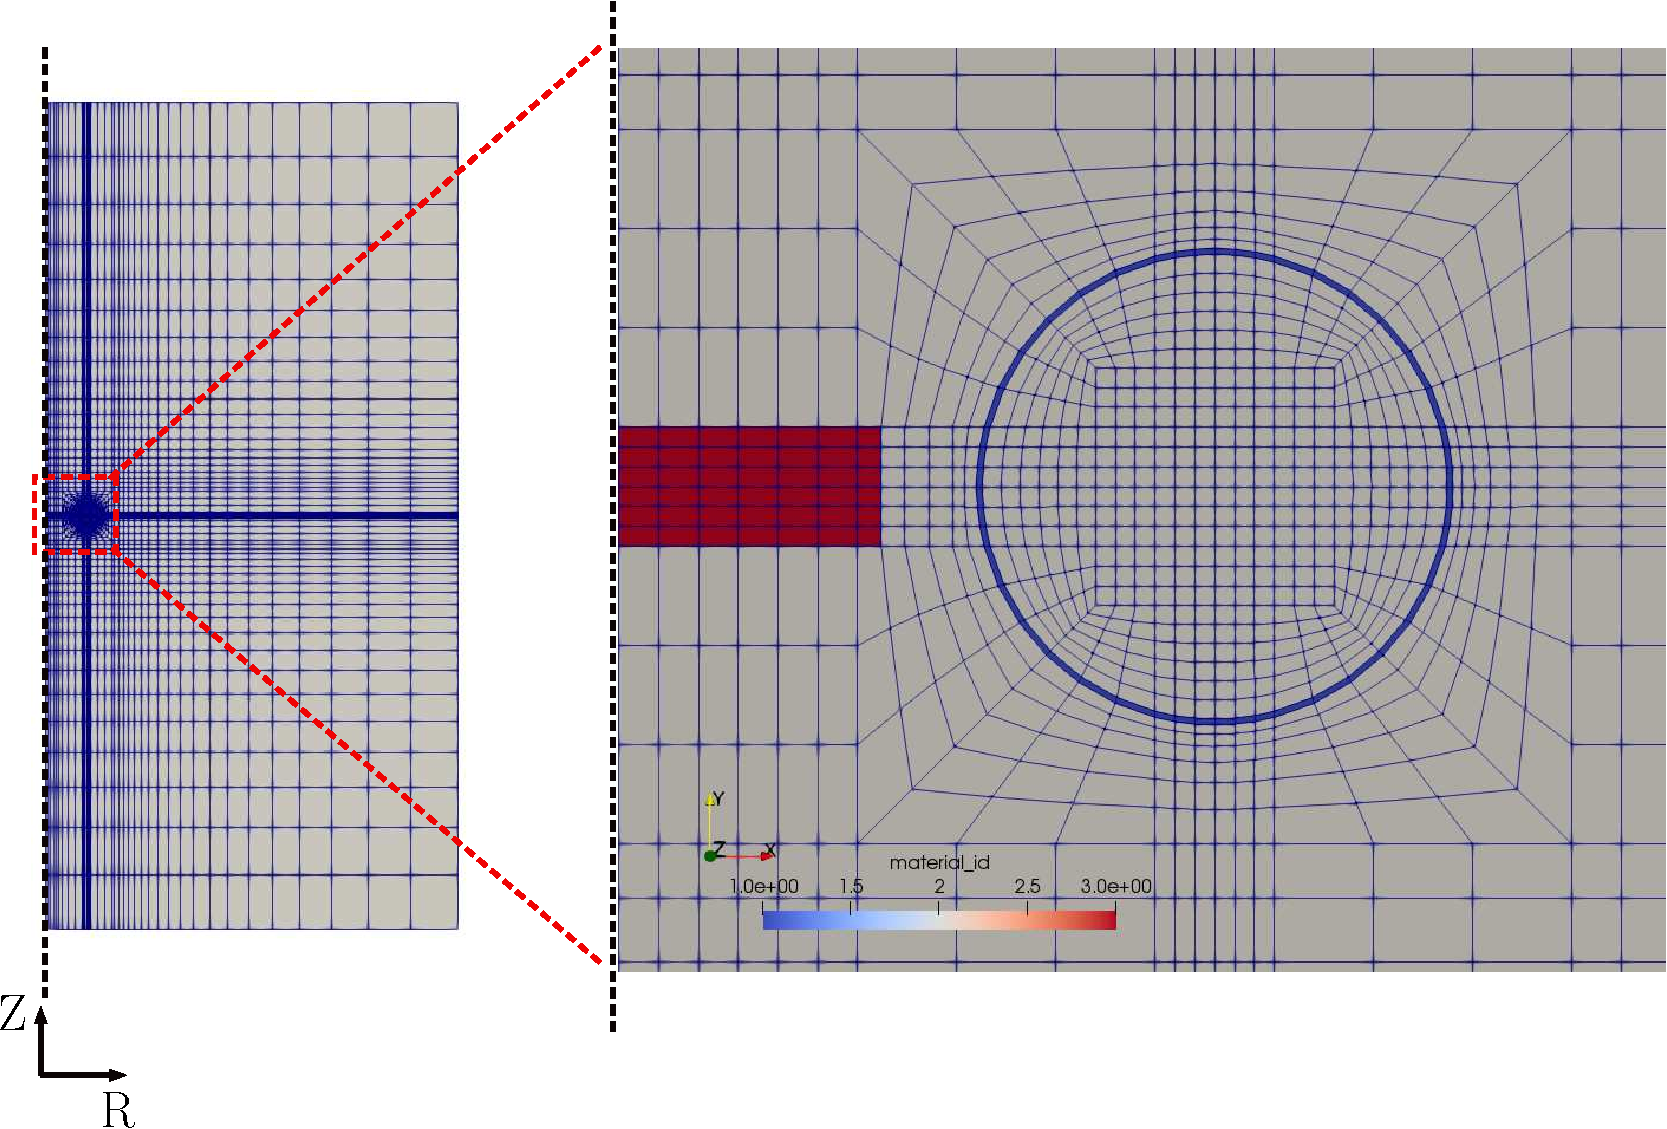
\includegraphics[width=0.7\textwidth]{2d_mesh.pdf}
\caption{Axisymmetric (2.5D) mesh geometry of toroid tube material modelled with surrounding free space (Red region: permanent magnet, blue region: torus magneto-elastic material and remaining region is the free space)}
\label{fig:1.2}
\end{figure}

\begin{figure}[htb]
\centering
\begin{subfigure}[b]{0.39\textwidth}
\centering
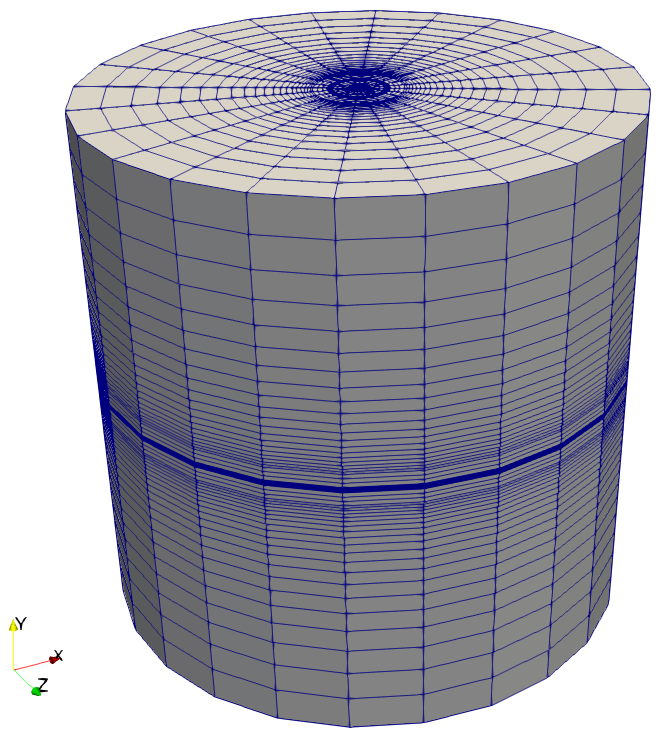
\includegraphics[width=0.9\textwidth]{3d_mesh_1.png}
\caption{3D mesh with free space}
\label{fig:1.3.1}
\end{subfigure}
\begin{subfigure}[b]{0.29\textwidth}
\centering
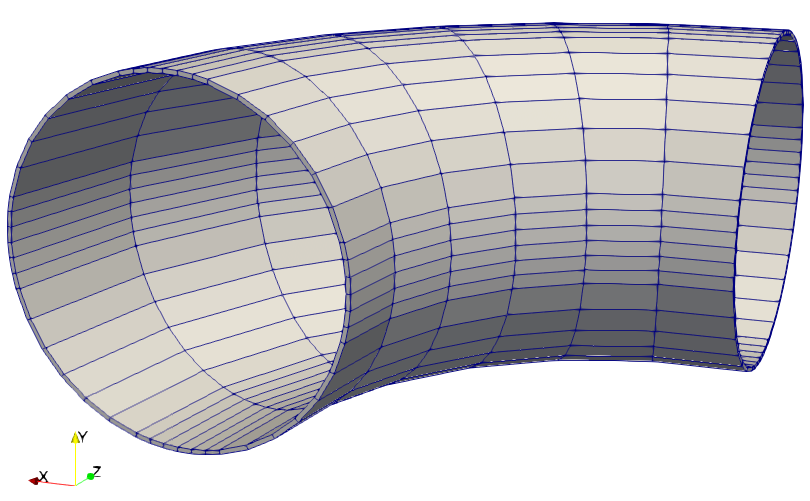
\includegraphics[width=0.85\textwidth]{3d_mesh_3.png}
\label{fig:1.3.2}
\caption{Cut section of toroid tube}
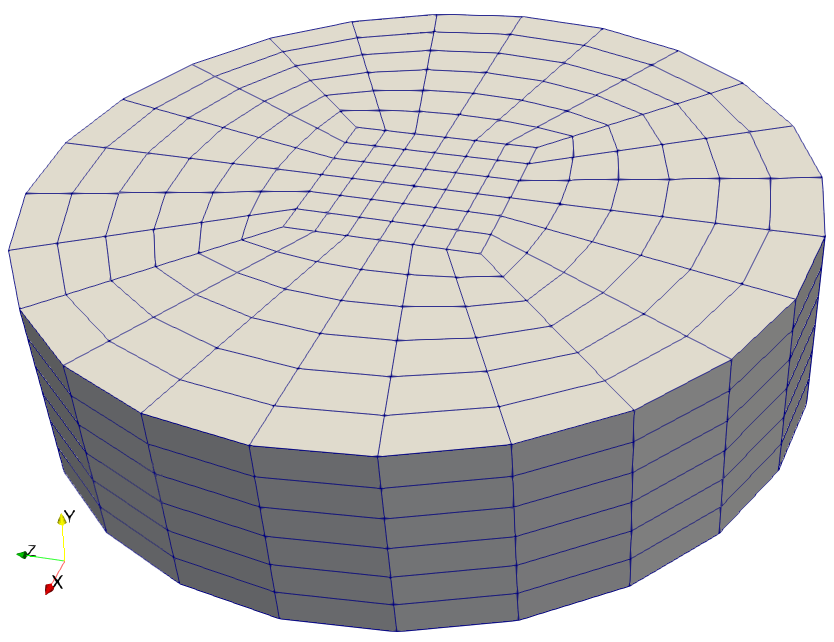
\includegraphics[width=0.85\textwidth]{3d_mesh_5.png}
\caption{Permanent magnet region}
\label{fig:1.3.4}
\end{subfigure}
\begin{subfigure}[b]{0.29\textwidth}
\centering
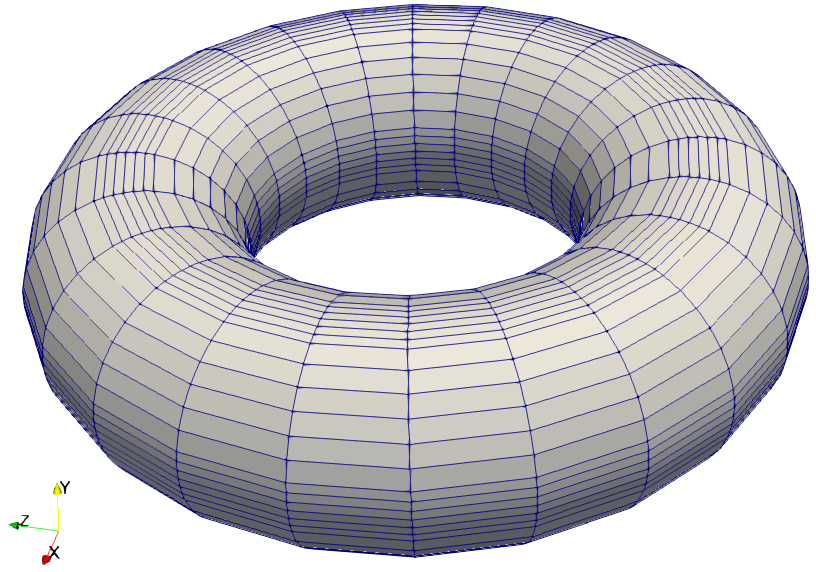
\includegraphics[width=0.75\textwidth]{3d_mesh_4.png}
\caption{Toroid tube}
\label{fig:1.3.3}
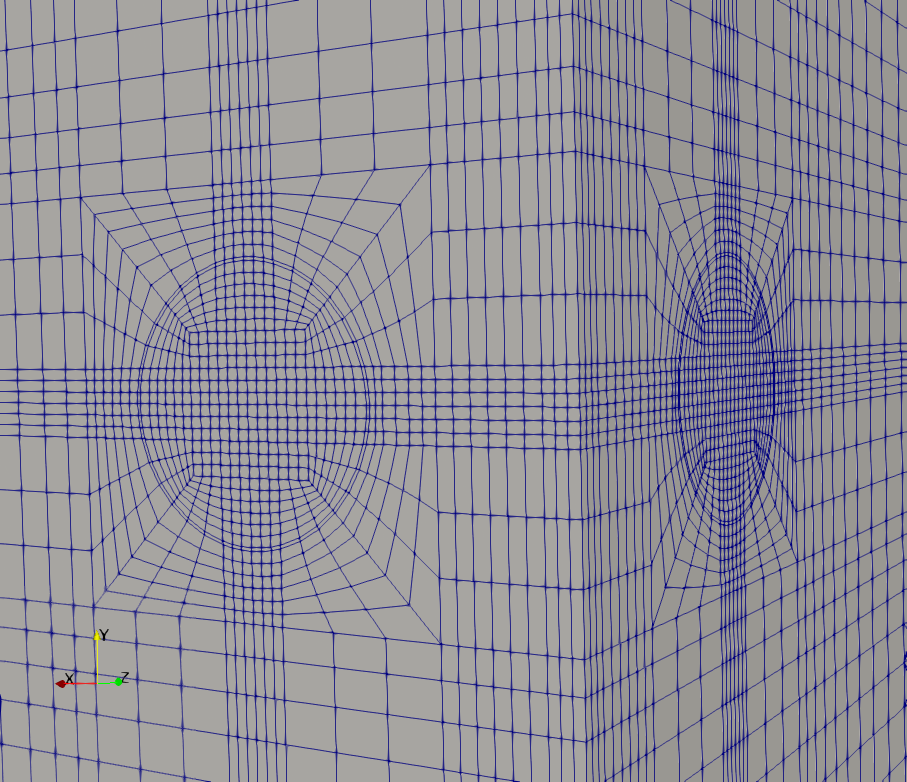
\includegraphics[width=0.75\textwidth]{3d_mesh_6.png}
\caption{Zoomed cross-section}
\label{fig:1.3.5}
\end{subfigure}
\caption{3D mesh geometry}
\label{fig:1.3}
\end{figure}

\section{Implementation details}
The open-source, high performance finite element library deal.II \cite{BangerthHartmannKanschat2007,dealII90} is used to model and simulate the magneto-elastic material with the free space around the toroid tube. Trilinos \cite{trilinos} vectors, matrices, preconditioners and solvers are used. The use of class  \href{https://www.dealii.org/current/doxygen/deal.II/classparallel_1_1shared_1_1Triangulation.html}{parallel$::$shared$::$Triangulation} for automatic partitioning of the domain among all the involved MPI processes (in parallel context) is done. To perform adaptive h-/p-refinement of the coarse mesh for a certain number of refinement iterations we employ the class \href{https://www.dealii.org/current/doxygen/deal.II/classhp_1_1DoFHandler.html}{hp$::$DoFHandler} to manage the distribution and enumeration of the degrees of freedom. In adaptive p-refinement we can have a different finite element on every cell of our mesh, whereas in h-refinement we can reduce the size of the mesh element where the error in solution is large. To mark the fraction of cells with largest error that would be then refined, we use the standard Kelly error estimator from the literature which is suitable and efficient for a large class of elliptic PDE's including the Laplace problem that we solve here. \par 
To generate a circulating magnetic field around the toroid tube we apply a linearly varying potential function to a region at the center of the body. This region of constrained degrees of freedom with the potential values has a shape of a rectangular box (in 2D), see the red box region in Figure \eqref{fig:1.2} or circular disk (in 3D) at the center of the domain, see Figure \eqref{fig:1.3.4}. The dimensions for this permanent magnet box/disk region to constrain the degrees of freedom and the linear potential function with which these DoFs will be constrained are user input parameters. \par 

\section{Numerical results}
\subsection{Validation of the axisymmetric formulation}
In order to validate the results of the axisymmetric formulation with the 3D simulation results we compute and compare an energy metric (scalar) contained in the magneto-elastic toroid tube material. The energy is computed as
\begin{equation}
E = \sum\limits_{cells \in \mathcal{B}_{tube}} \sum\limits_{q} \frac{1}{2} \mu_0 \ \mu_r \ \alpha \ \norm{-\nabla \phi(q)}^2 \ J \ w(q),
\end{equation}
where $\alpha$ is the co-ordinate transformation scaling factor which has the value of $2 \pi r$ for the axisymmetric formulation (2.5D) and 1 for the 3D simulation.\par 

\begin{figure}[t!]
\begin{subfigure}[t]{0.49\linewidth}
\centering
\resizebox{\linewidth}{!}{
\begin{tikzpicture}
\begin{semilogxaxis}[
xlabel = $\text{Number of cells}$,
ylabel = $\text{Total energy in membrane}$,
%grid =both,
%grid style=dashed,
%minor grid style ={gray!30},
%major grid style ={gray!30},
%width=0.8\linewidth,
legend pos=north east,
]
\addplot[
color=red,
mark=square,
line width=1pt,
]
table[x=NumberOfCells,y=TotalEnergy]{ref_sol_2d_energy_ncells.dat};
\addlegendentry{Total energy}
\end{semilogxaxis}
\end{tikzpicture}
}
\caption{Axisymmetric formulation}
\label{fig:1.4.1}
\end{subfigure}
\begin{subfigure}[t]{0.46\linewidth}
\centering
\resizebox{\linewidth}{!}{
\begin{tikzpicture} 
\begin{semilogxaxis}[
xlabel = $\text{Number of cells}$,
%ylabel = $\text{}$,
%grid =both,
%grid style=dashed,
%minor grid style ={gray!30},
%major grid style ={gray!30},
%width=0.8\linewidth,
legend pos=north east,
]
\addplot[
color=red,
mark=square,
line width=1pt,
]
table[x=NumberOfCells,y=TotalEnergy]{3d_3ref_energy_ncells.dat};
\addlegendentry{Total energy}
\end{semilogxaxis}
\end{tikzpicture}
}
\caption{3D simulation}
\label{fig:1.4.2}
\end{subfigure}
\caption{Total energy in the magneto-elastic toroid membrane for each refinement cycle}
\label{fig:1.4}
\end{figure} \par 

We observe the total energy in the magneto-elastic membrane due to the applied magneto-static magnetic scalar potential for the axisymmetric formulation for 4 refinement cycles in Figure \eqref{fig:1.4.1} and for the 3D simulation for 3 refinement cycles in Figure \eqref{fig:1.4.2} (less number of refinement cycles due to memory bottleneck with vastly growing number of cells). 4 MPI processes were employed to obtain the results. As can be observed, the total energy by both the approaches are comparable with a maximum relative error of 15\%. We observe a convergence in the total energy with each h-adaptive mesh refinement cycle. High computational cost for the 3D simulation is clearly observable when comparing the number of cells in the domain against the number of cells in axisymmetric (2.5D) simulation result. \par 

\subsection{Experiment with the permanent magnet region and the applied potential}
We carried out a study on the size of the permanent magnet region in which we constrain the DoFs to a linearly varying magnetic potential. This region, as explained earlier, is a rectangular box in 2D/circular disk in 3D. In addition to studying the behaviour of results on the dependence of the size of this magnet region, we also experimented with the change in the linear potential function values. The magnet region dimensions (length and height) and the potential function to apply are user input parameters and are varied in this study. This experiment was carried out for the axisymmetric (2.5D) model only.\par 

\begin{figure}[h]
\centering
\begin{subfigure}{0.32\textwidth}
\centering
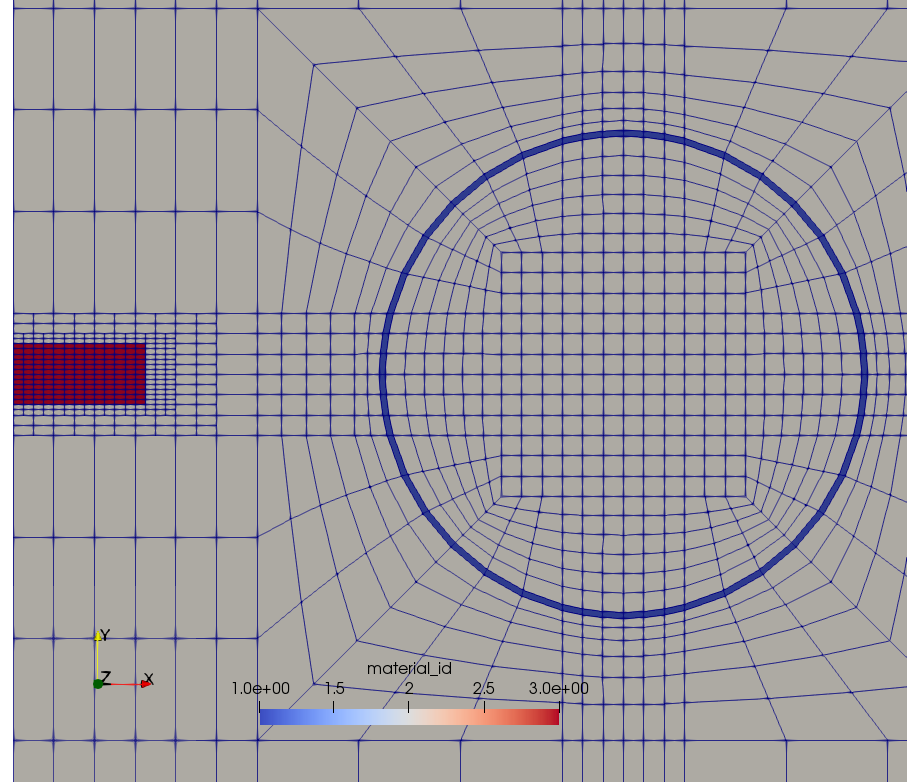
\includegraphics[width=0.87\textwidth]{magnet_x_p.png}
\caption{\scriptsize Magnet x=0.11,y=0.0255 \\(red block)}
\label{fig:1.5.1}
\end{subfigure}
\begin{subfigure}{0.33\textwidth}
\centering
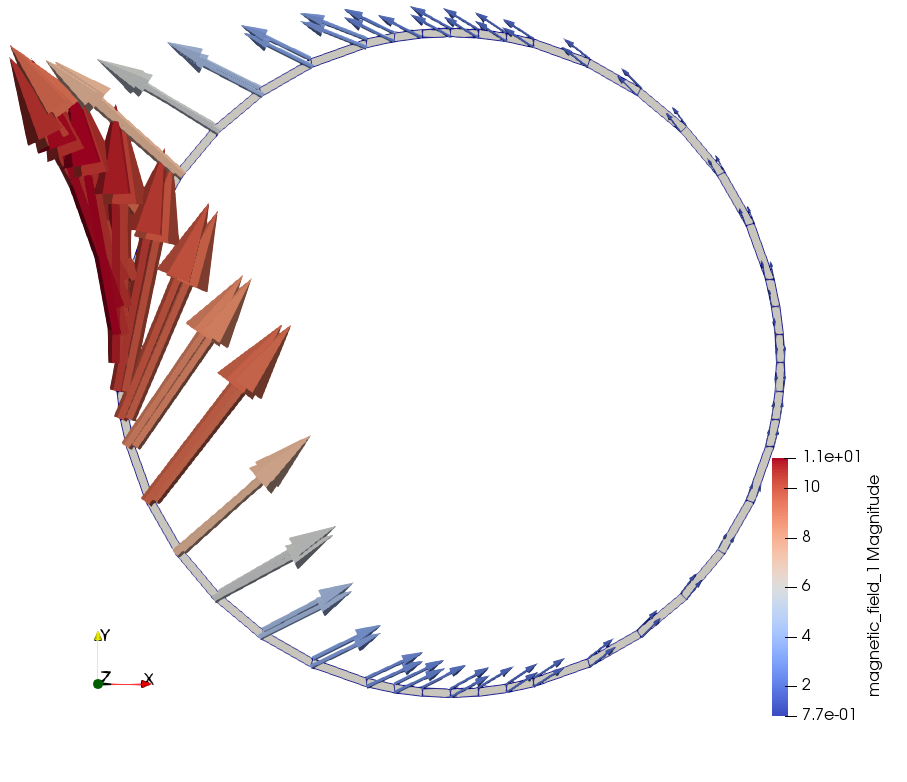
\includegraphics[width=0.85\textwidth]{x_p.png}
\caption{\scriptsize Pot. diff.= 1000 \\ Max. $\mathbbm{h}$= 1.1e+01, Min. $\mathbbm{h}$= 7.7e-01}
\label{fig:1.5.2}
\end{subfigure}
\begin{subfigure}{0.33\textwidth}
\centering
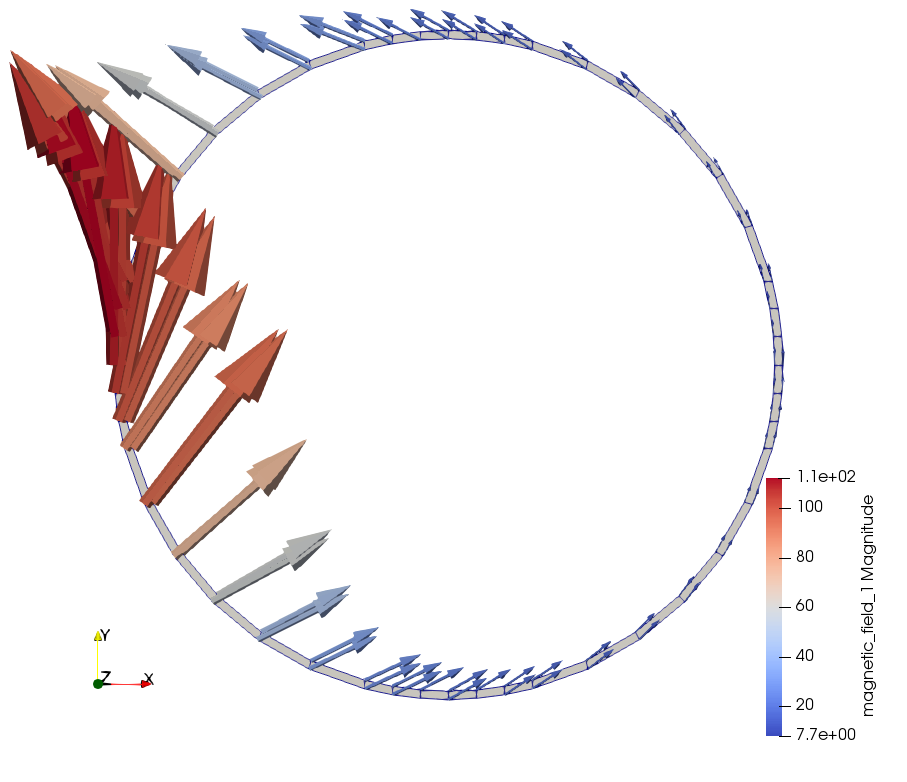
\includegraphics[width=0.85\textwidth]{x_10p.png}
\caption{\scriptsize Pot. diff.= 10000 \\ Max. $\mathbbm{h}$= 1.1e+02, Min. $\mathbbm{h}$= 7.7e+00}
\label{fig:1.5.3}
\end{subfigure}
\vspace{0.5cm}
\begin{subfigure}{0.32\textwidth}
\centering
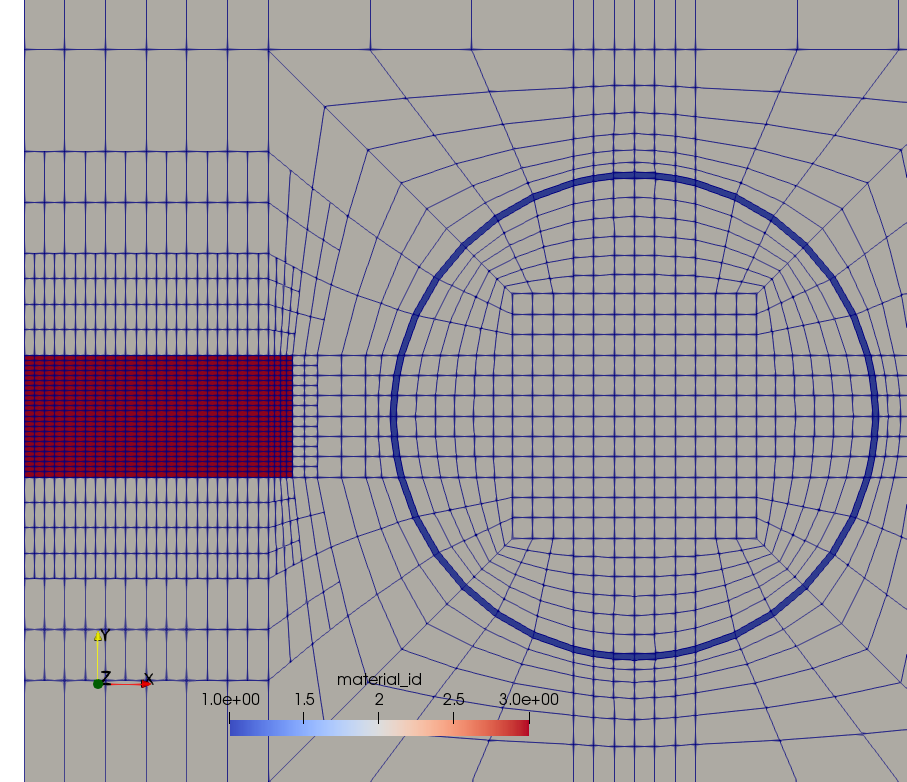
\includegraphics[width=0.87\textwidth]{magnet_2x_p.png}
\caption{\scriptsize Magnet x=0.22,y=0.051 \\(red block)}
\label{fig:1.5.4}
\end{subfigure}
\begin{subfigure}{0.33\textwidth}
\centering
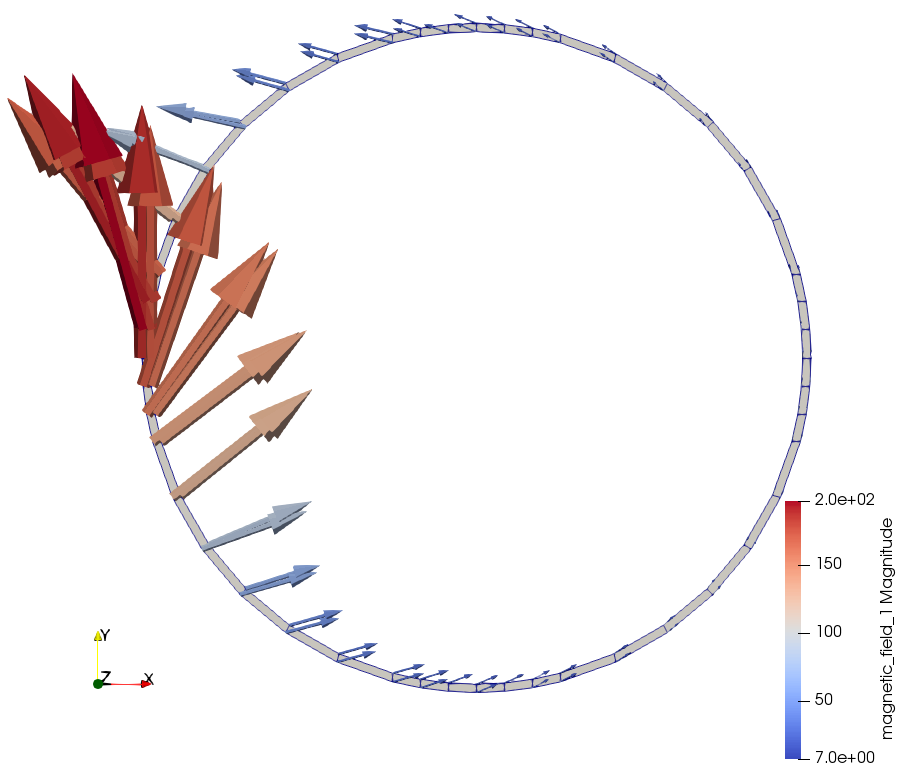
\includegraphics[width=0.85\textwidth]{2x_p.png}
\caption{\scriptsize Pot. diff.= 1000 \\ Max. $\mathbbm{h}$= 2.0e+02, Min. $\mathbbm{h}$= 7.0e+00}
\label{fig:1.5.5}
\end{subfigure}
\begin{subfigure}{0.33\textwidth}
\centering
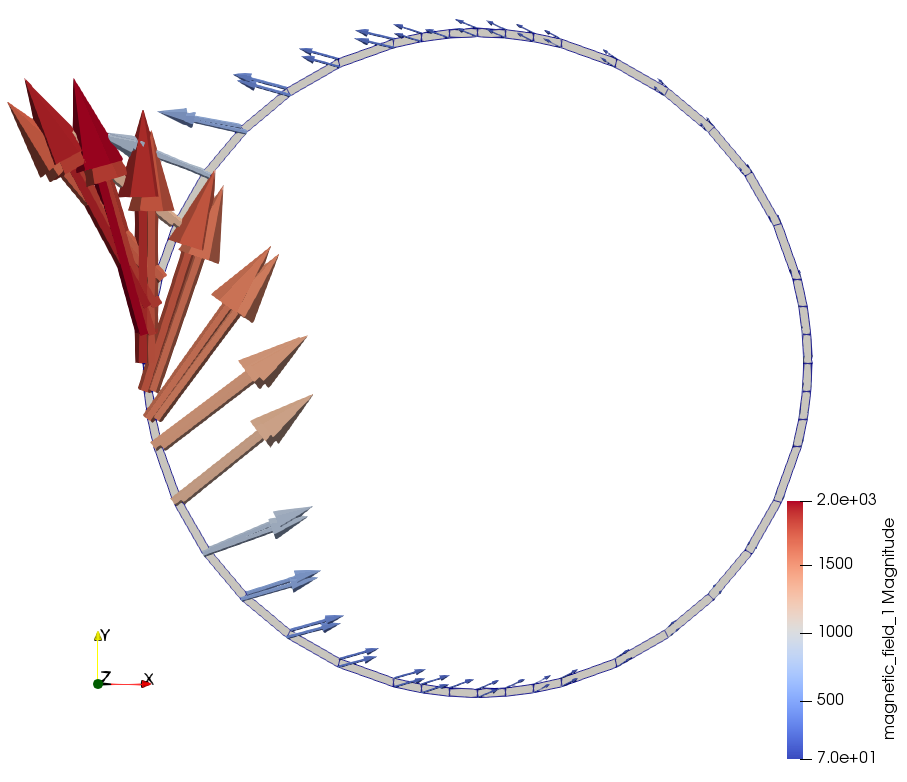
\includegraphics[width=0.86\textwidth]{2x_10p.png}
\caption{\scriptsize Pot. diff.= 10000 \\ Max. $\mathbbm{h}$= 2.0e+03, Min. $\mathbbm{h}$= 7.0e+01}
\label{fig:1.5.6}
\end{subfigure}
\caption{Effect of magnet size and applied magnetic potential in torus membrane field}
\label{fig:1.5}
\end{figure}

In the above figures we observe the resulting magnetic field $\mathbbm{h}$ for the input magnet region and applied magnetic potential parameters. Figure \eqref{fig:1.5.4} has double the magnet size when compared to the magnet size in Figure \eqref{fig:1.5.1}. When comparing the results for this effect of increased magnet size, we observe in Figure \eqref{fig:1.5.5} an increase in the magnitude of the magnetic field against the result in Figure \eqref{fig:1.5.2}. In Figure \eqref{fig:1.5.3} we increase the applied magnetic potential ten times of that used in the result for Figure \eqref{fig:1.5.2} keeping the size of the permanent magnet region the same. We observe the magnetic field has proportionally increased by same magnitude. Combined increase in the magnet region (twice as original size) and magnetic potential (10 times the original value) we observe the magnetic field has increased by a significantly large magnitude, see Figure \eqref{fig:1.5.6}. It is important to observe that the direction of magnetic field near the torus membrane did not change in any of the variation case. The aim of this study is to find appropriate values for the above three parameters such that we have a tangential magnetic field in the torus membrane to satisfy the curl free condition as given in Equation \eqref{eq:1.2}. \par 

The results with appropriately chosen values of these parameters for future work are depicted in Figure \eqref{fig:1.6} and \eqref{fig:1.7}.

\begin{figure}[h]
\centering
\begin{subfigure}{0.49\textwidth}
\centering
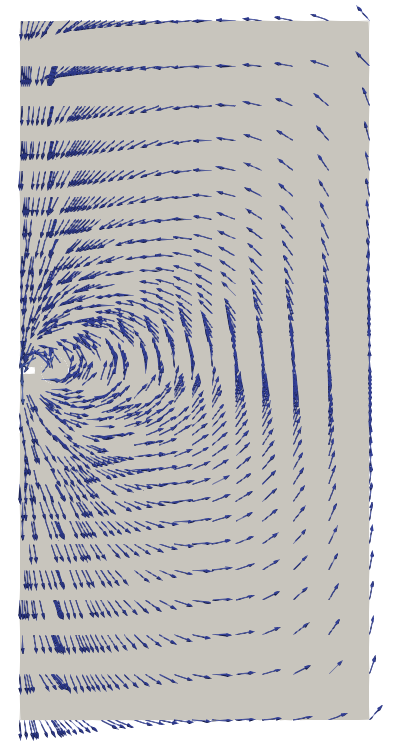
\includegraphics[width=0.55\textwidth]{2d_free_space.png}
\caption{Magnetic field in free space}
\label{fig:1.6.1}
\end{subfigure}
\begin{subfigure}{0.49\textwidth}
\centering
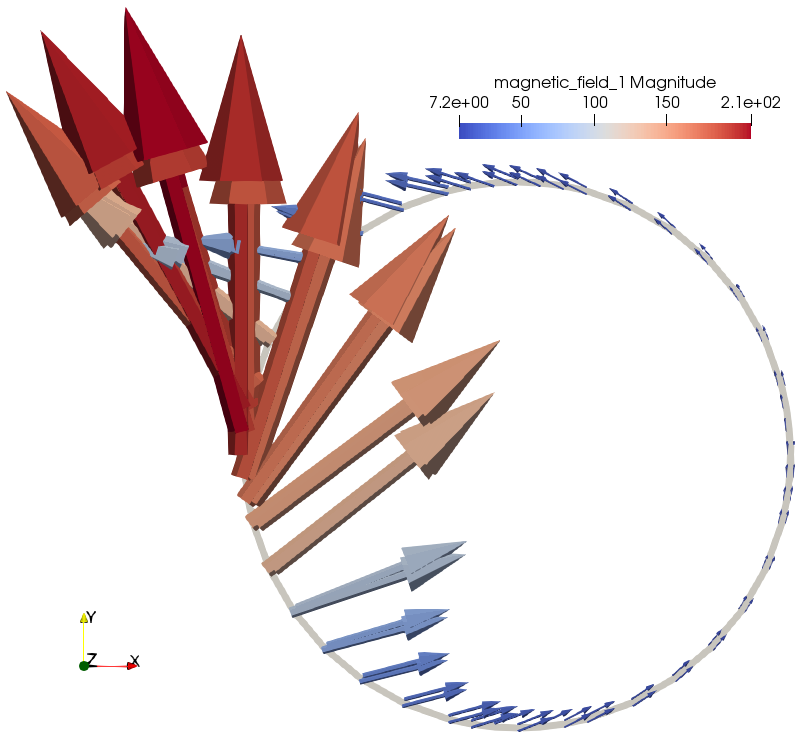
\includegraphics[width=0.85\textwidth]{2d_toroid_field_2.png}
\caption{Magnetic field in torus membrane}
\label{fig:1.6.2}
\end{subfigure}
\caption{Axisymmetric (2.5D) formulation}
\label{fig:1.6}
\end{figure}

\begin{figure}[h]
\centering
\begin{subfigure}{0.49\textwidth}
\centering
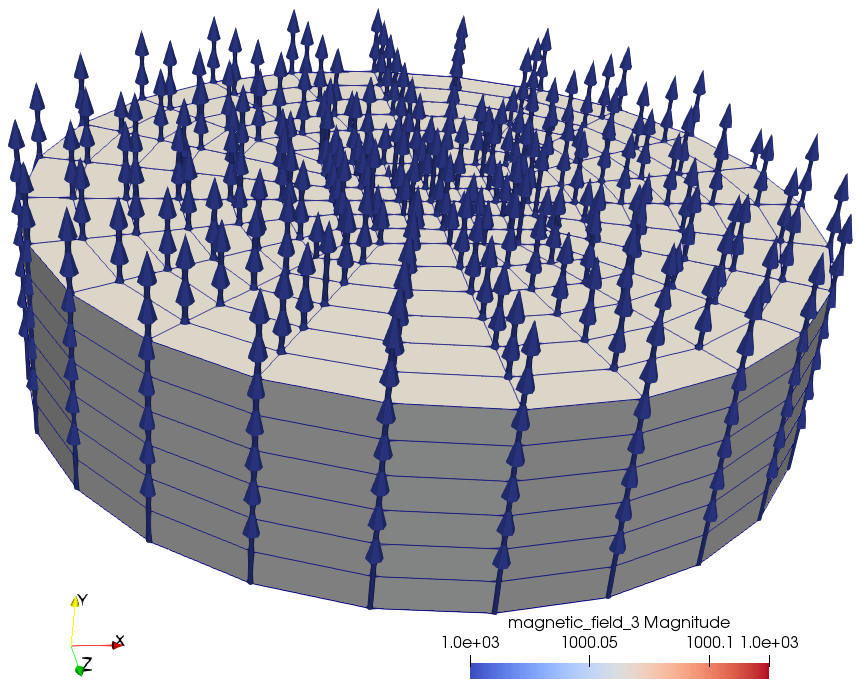
\includegraphics[width=0.8\textwidth]{3d_1quar_magnet_field.png}
\caption{Magnetic field in permanent magnet}
\label{fig:1.7.1}
\end{subfigure}
\begin{subfigure}{0.49\textwidth}
\centering
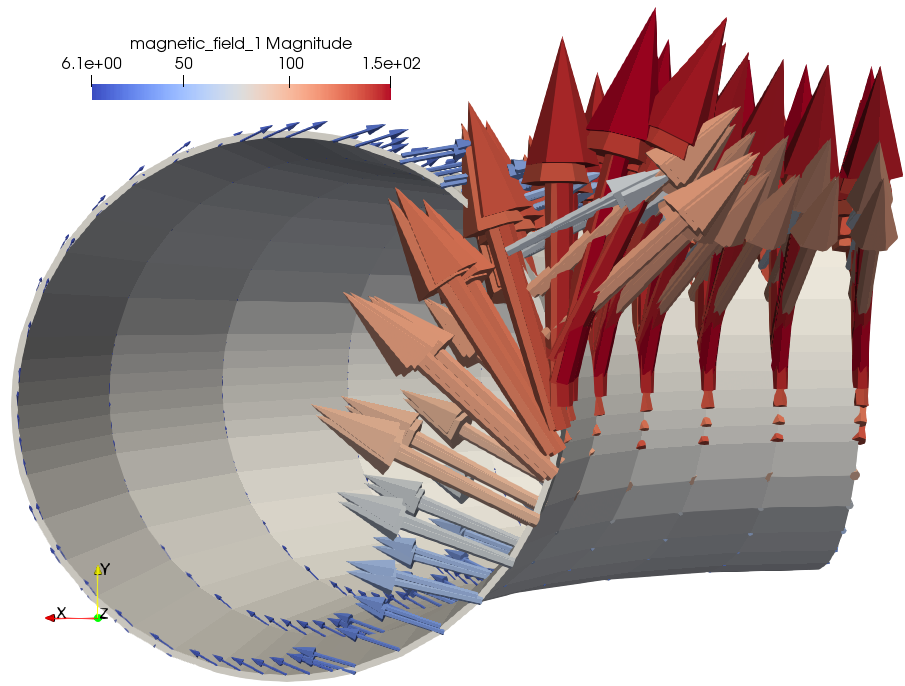
\includegraphics[width=0.85\textwidth]{3d_1quar_toroid_field_2.png}
\caption{Magnetic field in torus membrane}
\label{fig:1.7.2}
\end{subfigure}
\caption{3D simulation}
\label{fig:1.7}
\end{figure}
